\subsection{Tutor Availability}

\begin{figure}[H]
    \centering
    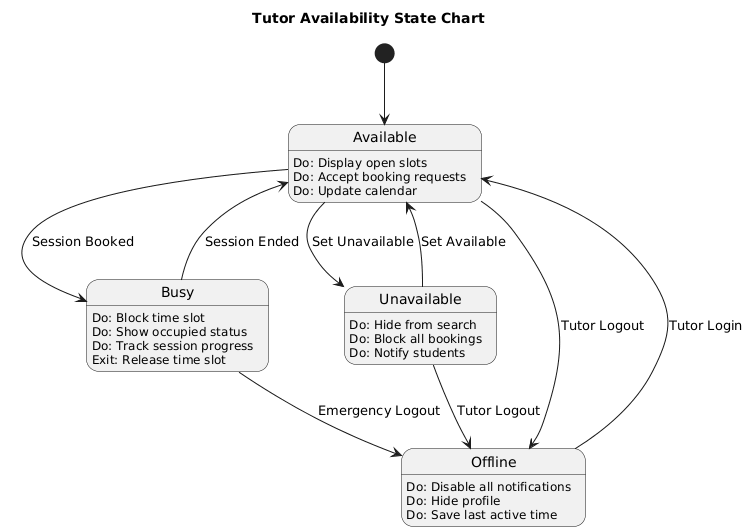
\includegraphics[width=\textwidth]{graphics/chapter5/tutor_avail.png}
    \caption{Tutor Availability}
    \label{fig:Tutor_Availability}
\end{figure}

\newpage

\noindent \textbf{Description}
\begin{itemize}
  \item \textbf{Purpose:} Model the availability status of a tutor throughout their active time in the system.
  
  \item \textbf{States:} 
    \textit{Available} (Do: Display open slots, Accept booking requests, Update calendar);
    \textit{Busy} (Do: Block time slot, Show occupied status, Track session progress);
    \textit{Unavailable} (Do: Hide from search, Block all bookings, Notify students);
    \textit{Offline} (Do: Disable all notifications, Hide profile, Save last active time).
  
  \item \textbf{Transitions:}
    Tutor Login $\Rightarrow$ \textit{Available};
    Session Booked $\Rightarrow$ \textit{Busy};
    Session Ended $\Rightarrow$ \textit{Available};
    Set Unavailable from \textit{Available} $\Rightarrow$ \textit{Unavailable};
    Set Available from \textit{Unavailable} $\Rightarrow$ \textit{Available};
    Tutor Logout from \textit{Available}, \textit{Unavailable}, or \textit{Busy} $\Rightarrow$ \textit{Offline};
    Emergency Logout from \textit{Busy} $\Rightarrow$ \textit{Offline}.
  
  \item \textbf{Start/End:} 
    Initial node $\rightarrow$ \textit{Available}; 
    \textit{Offline} can return to \textit{Available} (cyclic behavior).
  
  \item \textbf{Notes:} 
    Only \textit{Available} tutors appear in student searches; 
    \textit{Busy} tutors have their time slot blocked but remain visible; 
    \textit{Unavailable} tutors are hidden from search results;
    \textit{Offline} tutors have no active presence in the system;
    Tutors can toggle between \textit{Available} and \textit{Unavailable} manually;
    System automatically transitions from \textit{Busy} to \textit{Available} when session ends.
\end{itemize}
